\documentclass[conference]{IEEEtran}
%	\IEEEoverridecommandlockouts
\usepackage{cite}
\usepackage{amsmath,amssymb,amsfonts}
%	\usepackage{algorithmic}
\usepackage[dvipdfmx]{graphicx}
\usepackage{textcomp}
\usepackage{xcolor}
\definecolor{blue}{rgb}{0.00, 0.00, 1.00}
\usepackage{listings}
\usepackage{datetime2}
\usepackage{algorithm}
\usepackage{algorithmicx}
\usepackage{algpseudocode}
\def\BibTeX{{\rm B\kern-.05em{\sc i\kern-.025em b}\kern-.08em T\kern-.1667em\lower.7ex\hbox{E}\kern-.125emX}}
\lstset{
  language={Fortran},
  basicstyle={\ttfamily},
  identifierstyle={\small},
  %	commentstyle={\smallitshape},
  % keywordstyle={\small\bfseries},
  keywordstyle={\small},
  ndkeywordstyle={\small},
  %	stringstyle={\small\ttfamily},
  frame={tb},
  breaklines=true,
  columns=[l]{fullflexible},
  numbers=left,
  xrightmargin=0zw,
  xleftmargin=2zw,
  numberstyle={\scriptsize},
  stepnumber=1,
  numbersep=1zw,
  lineskip=-0.5ex,
  %	belowcaptionskip=10pt,abovecaptionskip=10pt
}


\begin{document}

\title{
\textcolor{blue}{as of \DTMnow} \\
Performance evaluation and visualization of scientific applications using PMlib
}

\author{
\IEEEauthorblockN{1\textsuperscript{st} Kazunori Mikami}
\IEEEauthorblockA{\textit{Flagship 2020 Project} \\
\textit{Riken R-CCS}\\
Kobe, Japan \\
kazunori.mikami@riken.jp}
\and
\IEEEauthorblockN{2\textsuperscript{nd} Kenji Ono}
\IEEEauthorblockA{\textit{RIIT} \\
\textit{Kyushu University}\\
Fukuoka, Japan \\
keno@cc.kyushu-u.ac.jp}
}

\maketitle

\begin{abstract}
Sustained computational performance of scientific applications on HPC systems
is often observed much lower than the maximum system performance.
Understanding this gap requires multi-perspective analysis, i.e., the system
architecture perspective to evaluate the characteristics of micro architecture
elements such as processor core and memory, and the applications perspective
to correlate the theoretical computation coded as the source program with the
computation workload produced by compilers.
The authors developed PMlib open source library to address such synthetic analysis.
PMlib provides the way to report the arithmetic workload counted manually from
the source code, as well as the actually executed system workload.
It also provides the detail utilization report of processor specific hardware
including the categorized SIMD instruction statistics, the layered cache
hit/miss rate, and the corresponding bandwidth up to memory,
which are captured via hardware performance counters (HWPC).
Using of PMlib, users can conduct synthetic analysis of the application
performance, and obtain the hint for further optimized execution of applications.
\end{abstract}

\begin{IEEEkeywords}
performance evaluation,
arithmetic workload,
system workload,
performance visualization,
open source library,
PMlib
\end{IEEEkeywords}



\section{Introduction}

The purpose of this research.
In the development and the productive phase of the scientific application,
the performance evaluation is frequently conducted on the target HPC systems.
in order to understand the performance characteristics
of the application on the target system, and to explore the possibility of
applying further optimization to the software for elapsed time reduction.

As the background, there is well known fact that 
the sustained computational performance of scientific applications on HPC
systems can be much lower than the theoretical maximum performance
expected from the system specification, depending on the type of applications.

\cite{cite-1-1}

There have been many prededing studies to account for this gap between
the achieved performance and the maximum performance, mostly from architecture
point of view,
some mentioning the difficulty of utilizing parallel arithmetic functional units,
some mentioning the locality of data residing on memory/cache hiererchy.

\cite{paper-bottleneck-analysis}

The performance is measured in the unit of conducted workload / elapsed time.
We should remind that the definition of workload measurement can vary,
usually chosen from one of the the followings,
the arithmetic workload defined by the applications in their source program,
and the system workload actually executed on HPC systems that is represented as
machine instructions which is measured with hardware performance counters (HWPC).
The difference in the performance based on these two workload definitions
can be significant as explained in the later section \ref{},
and is sometimes confusing to application users.

%	Obvious relational effect of job manager and the system workload is not
%	the focus of this paper.

PMlib has the functionality
to explicitly measure the arithmetic workload counted in the source program
using manually formulated argument, as well as the functionality
to automatically measure the HWPC event base workload,
thus providing users an option to compare the difference in workloads.

In measuring the HWPC events, PMlib utilizes PAPI \cite{} low level API.
PMlib has its own scheme to choose the related HWPC event sets and to sort out
the event statistics according to run time environment variables, making it
easier to extract the statistics of interest.
Choosing the correct set of events for specific processor type and
translating the accumulated counts into meaningful performance index can be
non-trivial work if without PMlib.

The output information from PMlib is a blocked text report based on
the time averaged performance statistics, by default.
It also produces the Open Trace Format \cite{} tracing file reflecting
the shorter interval statistics which can be read by Web browser
visualization tool TRAiL \cite{}.

In this paper, some examples of the difference between
the arithmetic workload and the system workload will be shown first.

Next, moving on to the performance measurement of the workload,
some examples of PMlib feature to read the performance characteristics
will be shown.

Finally, some examples of the performance analysis and optimization
will be shown indicating the merit obtained from 
multi-perspective analysis.

%	detecting the performance bottleneck ???

%%%%%%%%%%%%%%%%%%%%%%%%%%%%%%%%%%%%%%%%%%%
%%%%%%%%%%%%%%%%%%%%%%%%%%%%%%%%%%%%%%%%%%%

\section{Computational workload and Performance evaluation}
\subsection{user perspective performance}

{\color{blue} Choose workload terminology!!! arithmetic/application/system}

The term "computational workload" for scientific application developpers
is generally perceived as the total volume of arithmetic operations,
expressed by the formulas in the source code written in Fortran/C/C++.

The workload at this level can be simply represented as below:
%単純結合式%	Use Sigma symbol to simplify

%	\begin{align*}
%	\end{align*}
\begin{equation}
		Workload = \sum_{i=1}^{types} W_{ops}(i) \\
\end{equation}
where i represents the arithmetic operation type such as
1:add, 2:sub, 3:mult, 4:div, 5:max, 6:min, 7:sqrt, ...,
and W\_ops(i) is the corresponding number of arithmetic operations for i-th
arithmetic type such as
W\_ops(add),
W\_ops(sub),
W\_ops(mult),
W\_ops(div),
W\_ops(max),
W\_ops(min),
W\_ops(sqrt)


For example, the performance value "flops" reported from Linpack (HPCC)
\cite{}
is calculated based on above arithmetic workload formula
\ref{}
using terms of addition and multiplication only.

\begin{align*}
Gflops = N^{2} \times ( 2/3 * N + 3/2 ) \times 1.0^{-9} / Time 
\end{align*}

\begin{equation}
		Workload = \sum_{i=1}^{2} W_{ops}(i)
\end{equation}
where
\begin{math}
		W_{ops}(1) : add = 1/3 N^{3} + 3/4 N^{2}
		and
		W_{ops}(2) : mult = 1/3 N^{3} + 3/4 N^{2}
\end{math}

In the development phase of the HPC applications, practical developers
choose and deploy the numerical algorithm which require the least
amount of arithmetic operations through the scientific consideration,
aiming to reduce the elapsed time to obtain the desired simulation results.
The workload in this context is named arithmetic workload in this paper.

PMlib can be used to evaluate this arithmetic workload as explained
in the later section \ref{}.


the source code formulas are then compiled to corresponding assembly
instructions.
Each arithmetic statement is mapped to a sequence of multiple instructions.
We use "weight factor" to map the original arithmetic operations to the
generated instructions to quantify the relationship.
Assuming a simple "weight factor" constant w\_\* for each type of
arithmetic operations, 
the workload at this point can be represented as below:

% workload_{system}
\begin{align*}
%単純結合式%	Use Sigma symbol to simplify
workload_{weight} =
	w_{add}\times N_{add} + w_{sub}\times N_{sub} + w_{mult}\times N_{mult} \\
	+ w_{div}\times N_{div} + w_{max}\times N_{max} + w_{sqrt}\times N_{sqrt} + ...
\end{align*}

\begin{align*}
Performance = workload / Time 
\end{align*}

This workload formula is named application workload in this paper.
The application workload formula is a simple representation of the original
arithmetic and provides easy-to-understand relationship between the change
in the algorithm and the resulting change in the workload.

Under certain conditions
%	namely, the compiler choice and its optimization options,
PMlib can be used to help formulate this application workload as explained
in the later section \ref{}.

While formulating the workload in the form of
\ref{}
or
\ref{}
provides the general idea of the theoretical workload requirement by the
application, it is open difficult for casual applications to formulate
the workload. The other representation of workload will be shown in
the subsequent section.

\subsection{system perspective performance}

For many applications, it can be difficult to formulate
the application workload.
Even if composing the formula is possible, the mapping of "weight factor"
can be even more complex ,as described below.

Mapping mathematical functions to the native instructions
depends on not only the systems architecture but also the compiling software
and its optimization options.
%	mostly, the compiler choice and its optimization options,

There are multiple choices of available instructions for the same
arithmetic operation on modern processors.
The choice of instructions from scalar/vector syntax is made by
compiler optimization strategy, for example.
In vector, the degree of parallelism, i.e. width of simultaneous data
operation, with the effect of loop length is influential.
In scalar, data locality is influential.
Run time hardware behavior including out-of-order execution can not
be reflected to static "weight factor".

Now we look the workload and the performance from system perspective.

The fact that the actual numerical computation is accomplished by the
limited set of hardware components, and that the HWPC is available
on modern HPC systems, makes it more practical to obtain the HWPC statistics
and to analyze them for performance evaluation.

reflects the combination of the latency and the throughput of the instruction
of the particular application.

PMlib can be used for such purpose.

%
% Can add example of:
%	"arithmetic workload" from the source code
%	"application performance" read from assembly code
%	PMlib measured "HWPC performance"
%

%%%%%%%%%%%%%   Start from here... %%%%%%%%%%%%%%%

\subsection{micro architecture elements}
In system architecture perspective,
micro architecture elements, above all, the number of compute cores
in the processor, the degree of parallelism inside the core,
the depth of cache/memory hierarchy and the data move rate at each hierarchy
all have relational impact to how the machine instructions are executed,
thus leading to sustained computing performance.

\subsection{PMlib addresses it!}

It also provides the processor specific hardware utilization report
including categorized SIMD instruction statistics,
layered cache hit/miss rate, and the corresponding bandwidth upto memory.
It utilizes PAPI low level API for obtaining HWPC event statistics.


%%%%%%%%%%%%%%%%%%%%%%%%%%%%%%%%%%%%%%%%%%%%%%%%%%%%%%%%%%%%%%%%%%%%%%%%%%%%%%
%	以下は IJSP163 日本語
%%%%%%%%%%%%%%%%%%%%%%%%%%%%%%%%%%%%%%%%%%%%%%%%%%%%%%%%%%%%%%%%%%%%%%%%%%%%%%
\subsection {システム評価的観点での性能}
\label{subsection:system-perf}


Through appropriate APIs, HWPC statistics can be accessed. PMlib utilize
PAPI \cite{papi-1} low level API to accomplish this, and calculate the
computing workload from the executed instructions.
For example, Intel Xeon Skylake Gold \cite{skylake-1} processor
floating point operations can be derived from the HWPC event statistics
using the formula below. \ref{skylake-ops-1}


\begin{math}
fpsp1  : "FP\_ARITH:SCALAR\_SINGLE"; \\
fpsp4  : "FP\_ARITH:128B\_PACKED\_SINGLE"; \\
fpsp8  : "FP\_ARITH:256B\_PACKED\_SINGLE"; \\
fpsp16 : "FP\_ARITH:512B\_PACKED\_SINGLE"; \\
fpdp1  : "FP\_ARITH:SCALAR\_DOUBLE"; \\
fpdp2  : "FP\_ARITH:128B\_PACKED\_DOUBLE"; \\
fpdp4  : "FP\_ARITH:256B\_PACKED\_DOUBLE"; \\
fpdp8  : "FP\_ARITH:512B\_PACKED\_DOUBLE";
\end{math}
\begin{align*}
OP{hwpc} = fpsp1 + fpdp1 + 4.0*fpsp4 + 8.0*fpsp8 \\
	+ 16.0*fpsp16 + 2.0*fpdp2 + 4.0*fpdp4 + 8.0*fpdp8;
\end{align*}

Fujitsu FX100 processor, for example, has a different event symbols as below.
\par
\begin{math}
fpdp1  : "1FLOPS\_INSTRUCTIONS"; \\
fpdp2  : "2FLOPS\_INSTRUCTIONS"; \\
fpdp4  : "4FLOPS\_INSTRUCTIONS"; \\
fpdp8  : "8FLOPS\_INSTRUCTIONS"; \\
fpdp16 : "16FLOPS\_INSTRUCTIONS";
\end{math}
\begin{align*}
OP{hwpc} = fpdp1 + 2.0*fpdp2 + 4.0*fpdp4 \\
	+ 8.0*fpdp8 + 16.0*fpdp16; 
\end{align*}

We call the workload measured in this fashion as HWPC workload,
and the evaluated performance as HWPC performance.
HWPC performance is frequently used in the 


The situation that the arithmetic performance, i.e. user perspective,
of scientific applications on HPC systems is low,
even if the HWPC performance, i.e. system perspective, is high
actually exhibits the difference of the workload definition as described above.


\section{PMlib}

\subsection {about PMlib}

PMlib is an open source library to monitor the scientific applications
performance.
\cite{PMlib2:webpage} \par

PMlib can measure two types of workload, i.e. arithmetic and HWPC.
Users insert the PMlib start/stop API statements in the source code.
Each measuring section has minimal properties such as name, type of operation,
exclusiveness, and the workload value.
The report from PMlib is classified into threads, processes, sections,
depending on the controlling environment variable.


\subsection {PMlib API}
PMlib API can be called from C++ and Fortran programs as below.

% \begin{lstlisting}
% \begin{lstlisting}[label={caller-f},captionpos=t]
\begin{lstlisting}[caption={using PMlib in Fortran program}]
program main
call f_pm_initialize (Nsections)
call f_pm_setproperties ("section1" icalc, iexcl)
call f_pm_start ("section1")
call MyComputation (fops)
call f_pm_stop ("section1", fops, ncall)
call f_pm_print ("", isort)
call f_pm_printdetail ("", ilegend, isort)
end
\end{lstlisting}


\subsection {choosing workload type}
If the arithmetic workload must be measured,
PMlib API pair start/stop accepts argument holding the value or the formula
of the workload contained inside the section sandwiched by start/stop.
The API accumulates the volume of workload internally towards its report.

If HWPC workload must be measured,
PMlib automatically detects the type of hardware, and reads the HWPC
event statistics at each of start/stop API.
In HWPC workload mode, PMlib does not use the argument value, if given any.
The choice of arithmetic workload or HWPC workload is made by a
run time environment variable HWPC\_CHOOSER.

Possible choice of HWPC\_CHOOSER value:

FLOPS \textbar BANDWIDTH\textbar VECTOR\textbar CACHE

While PAPI has a good set of user APIs and is well documented,
it is not a simple task to choose the correct native event sets and masks
of the specific target HPC processor type and to sort out the event values for
a desired performance category using a limited set of HWPC.
For example,
the standard output from papi\_native\_avail command on a server with
Intel Skylake Gold processor gives 5000+ lines.

PMlib takes the role to interface the application developer's intent to
categorize the performance with the raw information from HWPC, and to
help evaluate the performance.


Once PMlib APIs are coded in the application, PMlib preserves the HWPC
portability. That is, PMlib chooses and reads the appropriate HWPC event
set, if the application is run on different HPC systems.


%	PMlib report example 1


%	PMlib report example 2


%	PMlib report example 3



\subsection{PMlib internal timer}
PMlib is a portable open source package, and utilizes linux standard timer
gettimeofday by default. It also has the installation option to utilize
a system specific high resolution low overhead timer for several platforms.
The two HPC systems in the previous section have such timer, and PMlib has
provision to use them.
Fig \ref{fig:precise-timer} shows the comparison of standard timer and
high resolution timer on these system.


\begin{figure}[bt]
\centering
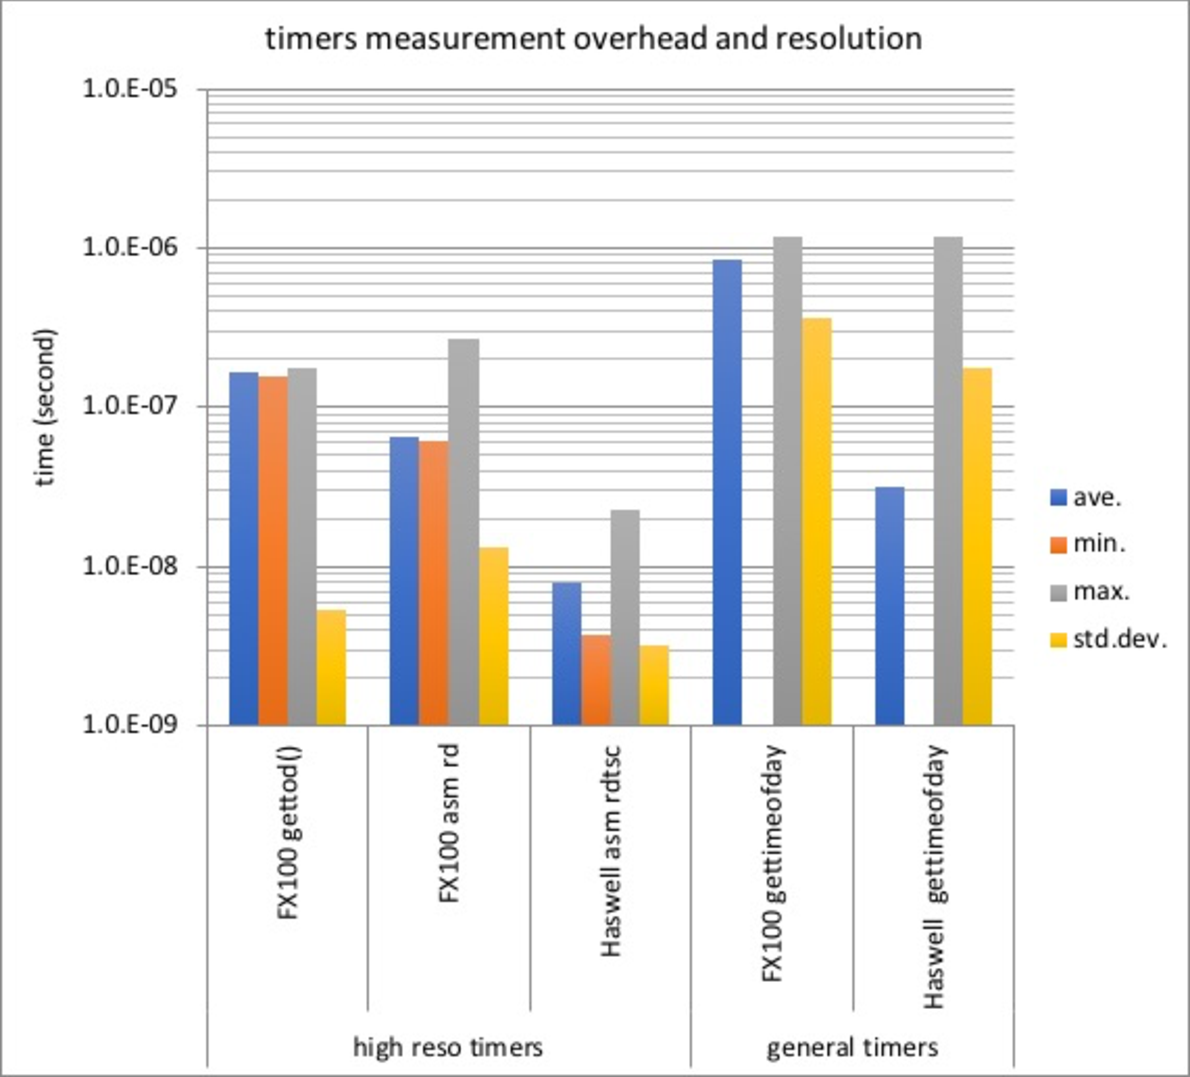
\includegraphics[width=0.45\textwidth]{figs/precise-timer.pdf}
\caption{precise-timer}
\label{fig:precise-timer}
\end{figure}



\subsection{PMlib output information}

{\color{blue} Maybe duplicated???}

The output information from PMlib is a blocked text report based on
the time averaged performance statistics, by default.
It also produces the Open Trace Format \cite{} tracing file reflecting
the shorter interval statistics which can be read by Web browser
visualization tool TRAiL \cite{}.


\subsection{other performance evaluation tools and related research}

There has been various tools developed for HPC system  performance evaluation.

In the open source category:
\begin{itemize}
	\item Scalasca \cite{Scalasca:2017} : trace generation, Score-P common
	infrastructure
	\item Extrae \cite{Extrae:webpage} :  trace generation
	\item PAPI \cite{PAPI:5.6} : API to access HWPC
	\item Linux perf tools : API to access HWPC
\end{itemize}

In the vendor supplied X86 category:
\begin{itemize}
		\item Intel VTune \cite{Intel:VTune}, PGI Profiler \cite{PGI:Profiler}
\end{itemize}

HPC systems also have the performance evaluation tools provided by the
system vendors.
Each of the tools has its own cons and pros.
The system vendor provided tools are integrated and qualified in general,
but is available on the vendor's HPC systems only.

The open source tools are designed to be portable. The functionality of the
tools are distinct, and multiple tools are used in sequence to obtain
the desired performance information.

These existing tools all utilize the processor performance information
based on HWPC workload, i.e. system workload.
PMlib appears to be the only tool that enables arithmetic workload
evaluation.



\section{PMlib use case}


Some examples of using PMlib for performance evaluation are shown in this
section.
The servers used for the measurements and their processor specifications
are listed in table \ref{tab:server-config}.

\subsection{measured HPC systems}

\begin{itemize}
{
%	\setlength{\itemsep}{-5pt}
%	\setlength{\topsep}{2mm}
\item SGI Intel Ivybridge server
\item SGI Intel Skylake server
\item Fujitsu prime HPC FX100
}
\end{itemize}


\newif\ifTwoservers
\newif\ifThreeservers
\Twoserversfalse
\Threeserverstrue
%\tiny
%\footnotesize
%\small
\begin{table}[b]
\scriptsize
\caption{server configuration and maximum performance}
\label{tab:server-config}
\footnotesize

\ifTwoservers
\begin{tabular}{l|c|c} \hline
\scriptsize
system			&	FX100	&	Skylake	\\ \hline
CPU				&	SPARC64 XIfx	&	Gold 6148	\\ \hline
core GHz		&	1.975	&	2.4	\\ \hline
core Gflops	&	31.6	&	〜30	\\ \hline
L1\$ size (D,I)		&	64KB, 64KB	&	32KB, 32KB	\\ \hline
L1D\$ BW GB/s	&	140/R+70/W	&	154/R + 77/W	\\ \hline
\$ Linesize 	&	256B	&	64B	\\ \hline
L2\$ size		&	-	&	1MB	\\ \hline
L2\$ BW GB/s/core	&	-	&	154 ( ~70)	\\ \hline
LL\$ size		&	12MB	&	28MB(1.4MB/c)	\\ \hline
LL\$ BW GB/s/core	&	70/R+35/W	&	77 ( ~43)	\\ \hline
Memory			&	HMC(8x16Ls)	&	DDR4-2666	\\ \hline
Mem GB/s/[CMGcpu]	&	120/R+120/W	&	128	\\ \hline
\#cores/[CMGcpu]	&	16	&	20	\\ \hline
\end{tabular}
\fi

\ifThreeservers
\begin{tabular}{l|c|c|c} \hline
\scriptsize
Symbol			&	FX100	&	SKY		&	IVY \\ \hline
Platform		&	FX100	&	Skylake & Ivybridge\\ \hline
CPU				&	SPARC64 XIfx	&	Gold 6148	&	E5-4620v2	\\ \hline
core GHz		&	1.975	&	2.4	&	2.6 \\ \hline
core Gflops	&	31.6	&	〜30	\\ \hline
\#core/cpu*	&	16	&	20	&	8	\\ \hline
L1\$ size(D,I)		&	64KB, 64KB	&	32KB, 32KB	\\ \hline
L1D\$ BW GB/s	&	140/R+70/W	&	154/R + 77/W	\\ \hline
\$ Linesize 	&	256B	&	64B	&	64B	\\ \hline
L2\$ size		&	-	&	1MB	&	256KB	\\ \hline
L2\$ BW GB/s/c	&	-	&	154 ( ~70)	\\ \hline
LL\$ size		&	12MB	&	28MB	&	20 MB	\\ \hline
LL\$ BW GB/s/c	&	70/R+35/W	&	77 ( ~43)	\\ \hline
Memory			&	HMC(8x16Ls)	&	DDR4-2666	& DDR3-1600	\\ \hline
Mem GB/s/cpu*	&	120/R+120/W	&	128	\\ \hline
\#cores/cpu*	&	16	&	20	\\ \hline
\multicolumn{4}{l}{\scriptsize\hspace{5mm} remark. cpu* indicates processor or
CMG }\\
\end{tabular}
\fi

\end{table}


\subsection{evaluation of basic kernels}

Basic kernels composed of four basic arithmetic operations and square root
are evaluated first.
Fortran source program for the measuring kernels is shown below.

\begin{lstlisting}[caption={basic kernels}]
subroutine sub_add(a,b,c,n)
real a(n), b(n), c(n)  
do i=1,n
c(i)=a(i)+b(i)
end do
return
subroutine sub_fma(a,b,c,n)
real a(n), b(n), c(n)  
do i=1,n
c(i)=a(i)+b(i)*d
end do
return
subroutine sub_divide(a,b,c,n)
real a(n), b(n), c(n)  
do i=1,n
c(i)=b(i)/a(i)
end do
return
subroutine sub_sqrt(a,b,c,n)
real a(n), b(n), c(n)  
do i=1,n
c(i)=sqrt(a(i))
end do
return
\end{lstlisting}


These basic kernels are computed as single strided loops without dependencies,
and are expected to be efficiently processed taking advantage of parallel
execution pipelines and wide units.
In this paper, the term vectorization and SIMD are used sinonimously.

Computing time is measured for above subroutines many times.
After subtracting the calling overhead time,
the average computing time for each kernel is obtained.
Do loop cost is included in the average computing time.

This simple measurement gives reasonable value on small dedicated systems
which do not suffer from the purtubation influence caused by
other processes, shared file system, network with shared topology,
called noise.
On HPC systems, it is not easy to remove the noise
especially for small granularity computation time.

On user side, removing the noise can be tried through statistic approach,
such as
adding additional outer loop for repeated measurement, and filter out
the measurements whose value is out of standard deviation.


The figure \ref{fig:fx100-gflops-long-R8} shows the 
measurement of the basic kernels on FX100 system using the loop length of
\begin{math}
n=1,2,4,..,2^{26}
\end{math}

\begin{figure}[bt]
\centering
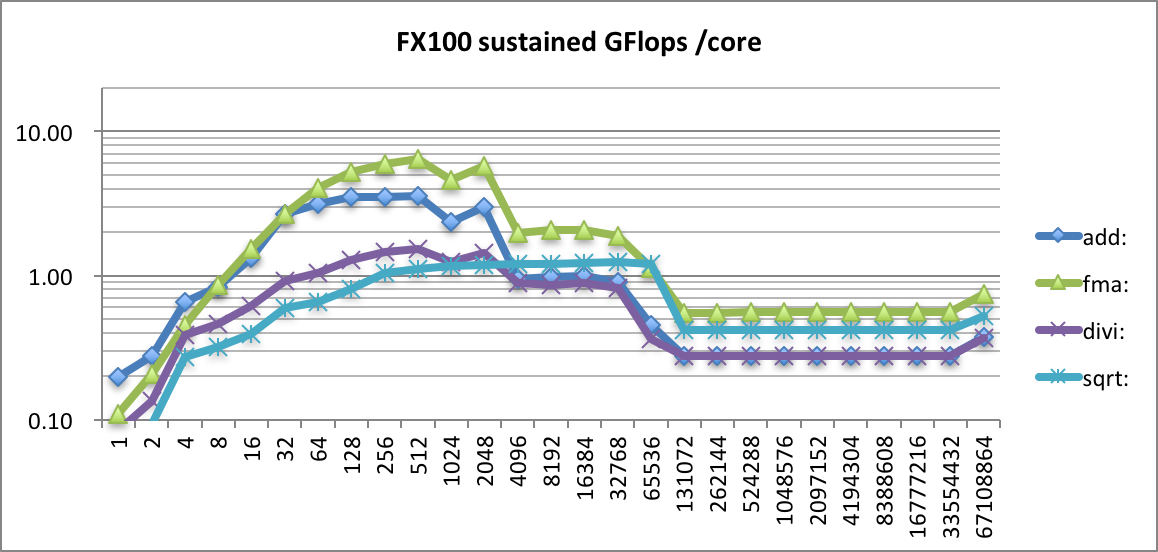
\includegraphics[width=0.45\textwidth]{figs/fx100-gflops-long-R8.pdf}
\caption{fx100-gflops-long-R8}
\label{fig:fx100-gflops-long-R8}
\end{figure}

The displayed curves represent arthmetic performance.
The performance tends to improve according to the increase of
loop length until L1 cache size limit is reached, and drops to
the bandwidth constrained performance level of the next level cash.
This performance tendency matches the reports from other associated research.

In short loop region,
the overhead to process loop set-up and update can not be neglected,
the the performance is bound to data access latency.

In long loop region,
the the performance is bound to
L1\$ / L2\$ / LLC / memory bandwidth in the roofline envelop.

\cite{Williams:2009:RIV:1498765.1498785} 

The figures
\ref{fig:fx100-gflops-short-R8} and \ref{fig:ivy-gflops-short-R8}
shows the detail performance characteristics of the same kernels
for
\begin{math}
n=1,2,3,..,128
\end{math}
and close-up look for
\begin{math}
n=1,2,3,..,50
\end{math}


\begin{figure}[bt]
\centering
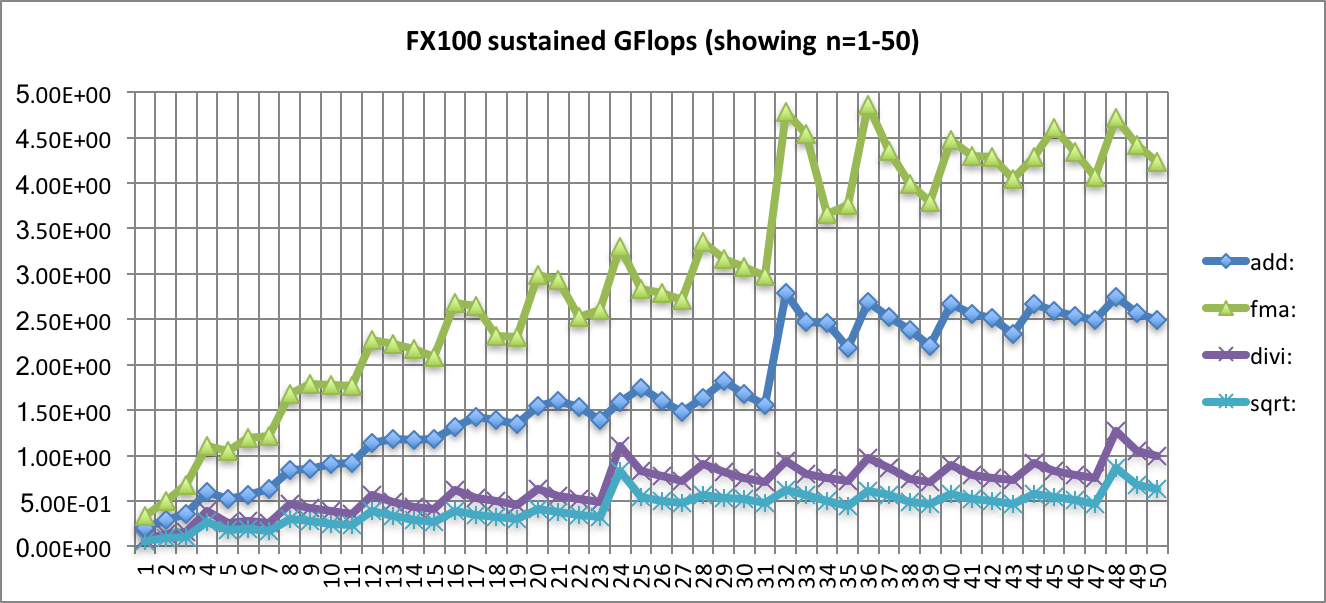
\includegraphics[width=0.45\textwidth]{figs/fx100-gflops-short-R8.pdf}
\caption{fx100-gflops-short-R8}
\label{fig:fx100-gflops-short-R8}
\end{figure}

\begin{figure}[bt]
\centering
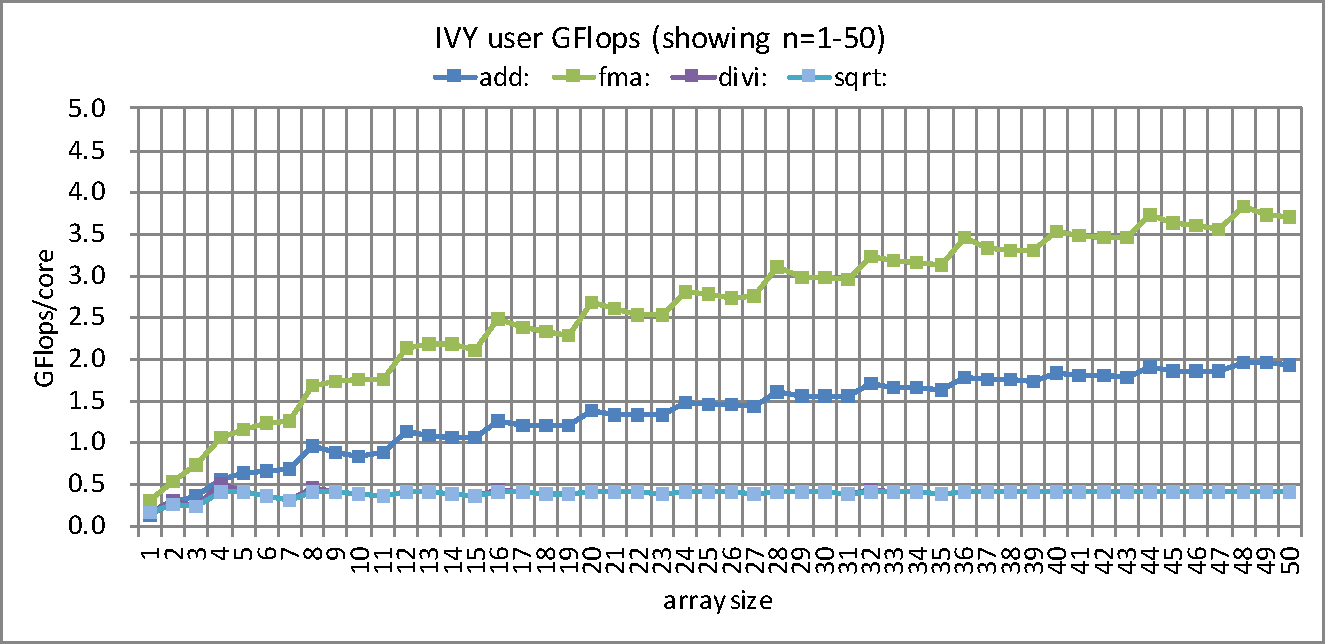
\includegraphics[width=0.45\textwidth]{figs/ivy-gflops-short-R8.pdf}
\caption{ivy-gflops-short-R8}
\label{fig:ivy-gflops-short-R8}
\end{figure}

The detail performance curves does not show gradual increase. Instead, they
show steep stepping shapes at multiple of constant interval.
This is a common observation on systems with SIMD supporting processors,
and the interval corresponds to the data width of SIMD instructions.
For example, FX100 double precision (64 bits) arithmetic can utilize
256 bit instruction, and the resulting interval is
\begin{math}
256 / 64 = 4
\end{math}
.
So the performance is highest at 4n, then 4n+1, 4n+2, and lowest at 4n+3.

The figure \ref{fig:fx100-gflops-short-R8} is showing the fact that
program coding practice to maintain the loop length as the multiply of
SIMD width has significant impact, especially for short loop computation.

The interval for single precision (32 bits) is
\begin{math}
256 / 32 = 8
\end{math}
, and shows even stronger performance impact as seen in figures
\ref{fig:fx100-gflops-short-R4} for FX100,
\ref{fig:HAS-gflops-short-R4} for Haswell CPU.

\begin{figure}[bt]
\centering
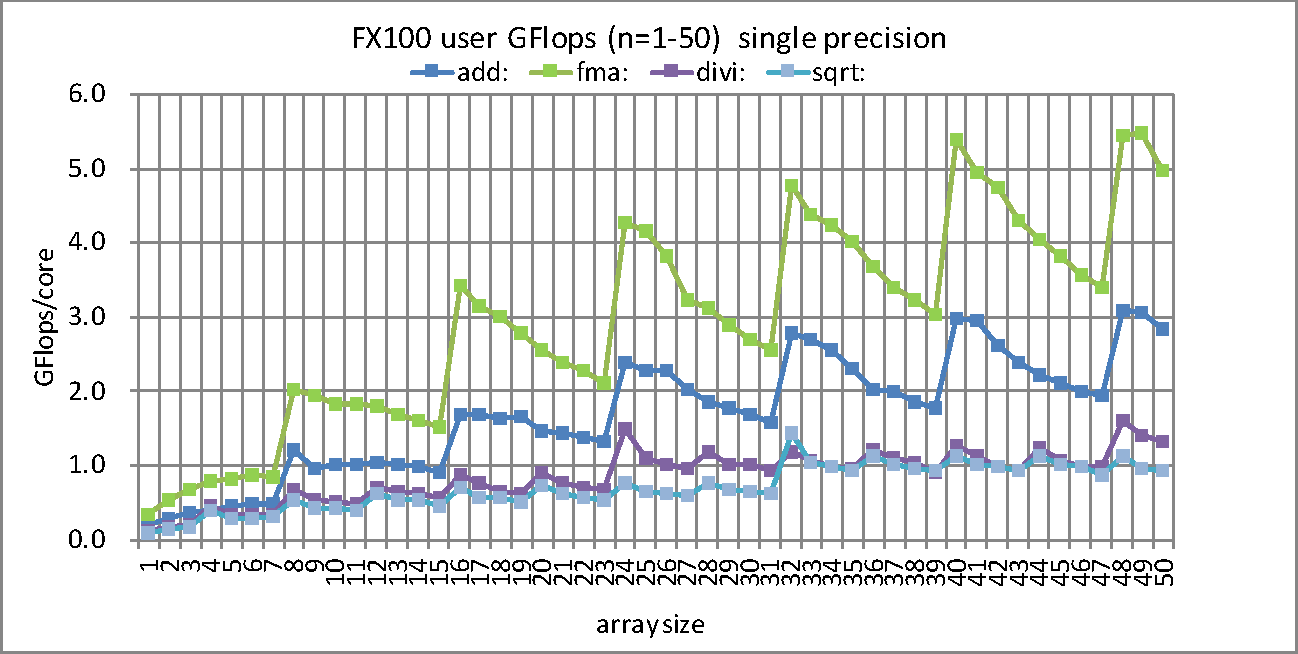
\includegraphics[width=0.45\textwidth]{figs/fx100-gflops-short-R4.pdf}
\caption{fx100-gflops-short-R4}
\label{fig:fx100-gflops-short-R4}
\end{figure}


\begin{figure}[bt]
\centering
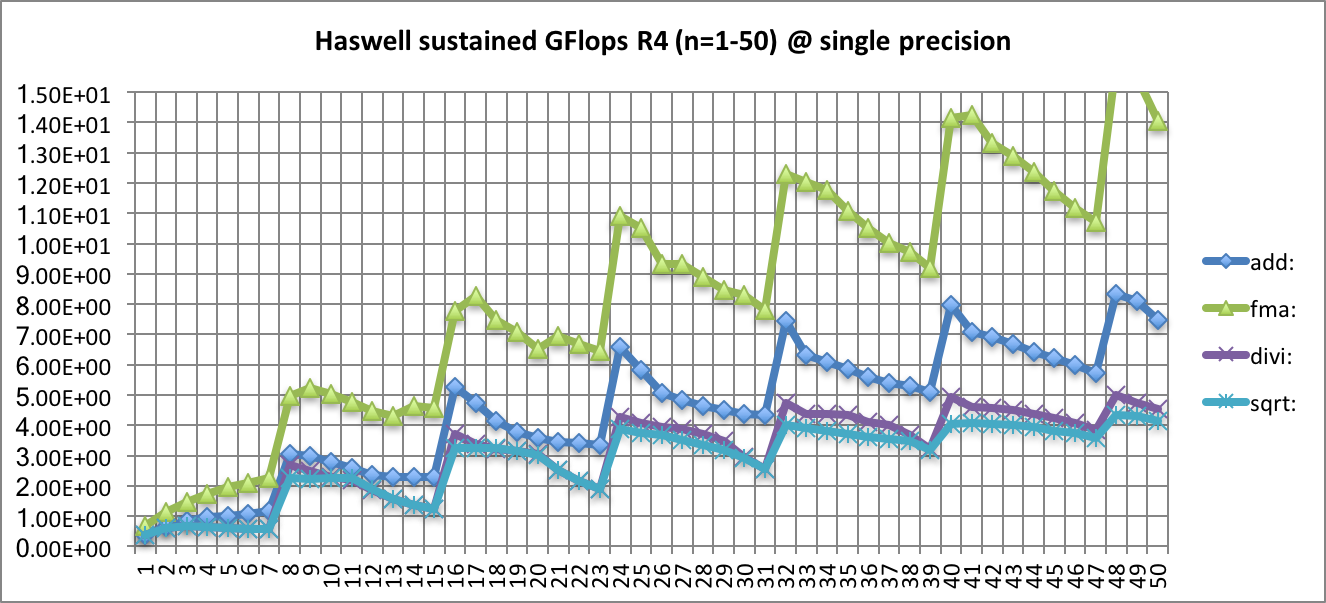
\includegraphics[width=0.45\textwidth]{figs/HAS-gflops-short-R4.pdf}
\caption{HAS-gflops-short-R4}
\label{fig:HAS-gflops-short-R4}
\end{figure}

Performance evaluation from the arithmetic perspective and from the
system perspective provides the capability to build up the theoretical
workload model of the application,
and the capability to map the model with the actual system workload
and performance on a specific HPC system.
PMlib provides the capability to conduct such synthetic performance
evaluation, and hopefully the hint for further optimized execution of
the application in its development and production phase.


\subsection{STREAM性能の評価}
STREAMベンチマーク\cite{stream:1995}
はコンピュータシステムのメモリバンド幅を測定するためのツールとして
広く用いられている.
STREAMは変数配列の積和算(TRIAD)など,メモリread/write処理が主要な負荷となる
計算式の性能をアプリケーションプログラムレベルで測定出力する.
したがってその結果は「計算科学的観点」で評価された性能である.
このSTREAMプログラムを「システム評価的観点」で評価するとかなり様相が異なる.

まずSTREAMをSkylakeサーバ上で実行した場合の出力結果を示す.
Intelコンパイラのデフォルトオプションを用いている.
STREAM FortranプログラムOpenMPスレッド並列版を
1CPU上で8スレッド実行した場合,20スレッド実行した場合について示す.

メモリ階層での実測イベントベースによるデータ移動の状況を示す.
図


Intelコンパイラにはオプションが多数あり,中でも特にメモリバンド幅に関係が深いと
思われる以下のオプションを組み合わせて比較した結果を
図\ref{fig:stream-ivy-compact-1cpux8} に示す.\\
{\color{blue}この図は仮置きでIvybridgeの結果.Skylakeの結果と差し替えること.}

\begin{figure}[bt]
\centering
%	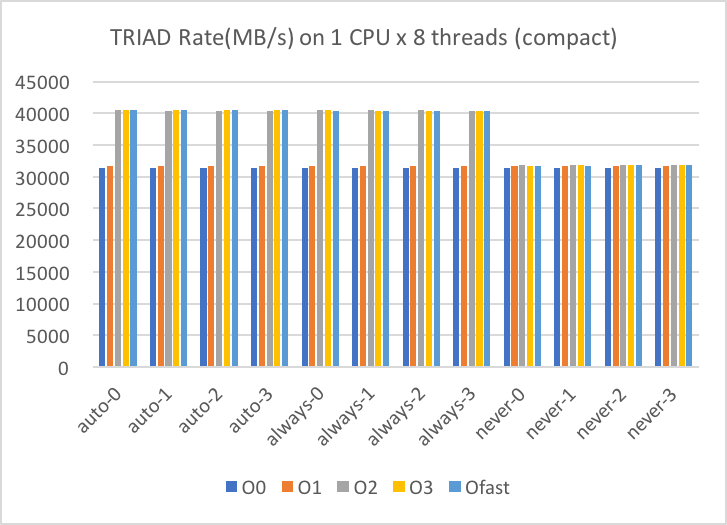
\includegraphics[width=0.45\textwidth]{figs/stream-ivy-compact-1cpux8.pdf}
\caption{stream-ivy-compact-1cpux8}
\label{fig:stream-ivy-compact-1cpux8}
\end{figure}


配列のファーストタッチなどデータの局所性確保,スレッドのコア固定など
を注意深く行うと,ノードに搭載された4CPUの全コアを使用した場合でも
同じような傾向の結果が得られる.
図\ref{fig:stream-ivy-scatter-4cpux8} に示す.\\

\begin{figure}[bt]
\centering
%	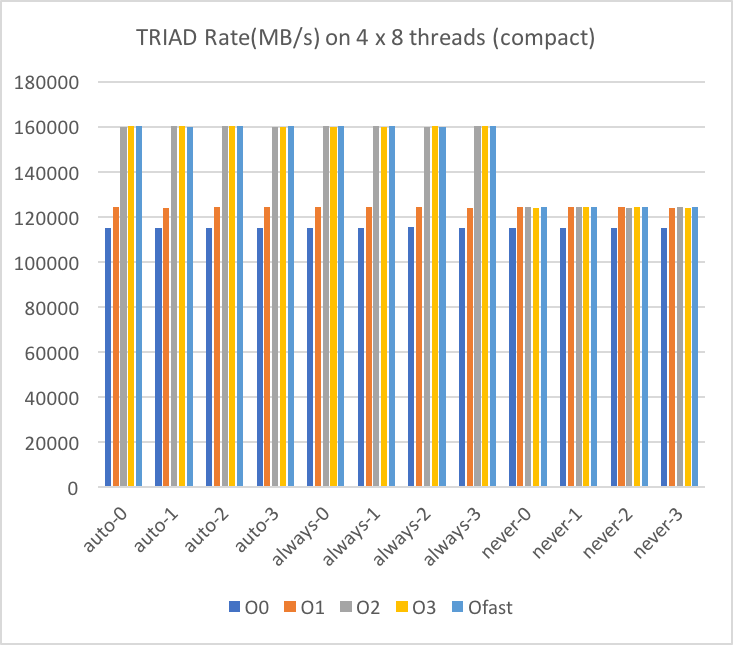
\includegraphics[width=0.45\textwidth]{figs/stream-ivy-scatter-4cpux8.pdf}
\caption{stream-ivy-scatter-4cpux8}
\label{fig:stream-ivy-scatter-4cpux8}
\end{figure}

これに対してアプリケーションのスレッド並列度が低い場合は様子が変わり,
例えばCPUあたり2スレッド(2コア)が実行されると
図\ref{fig:stream-ivy-scatter-4cpux2} の様になる.\\

\begin{figure}[bt]
\centering
%	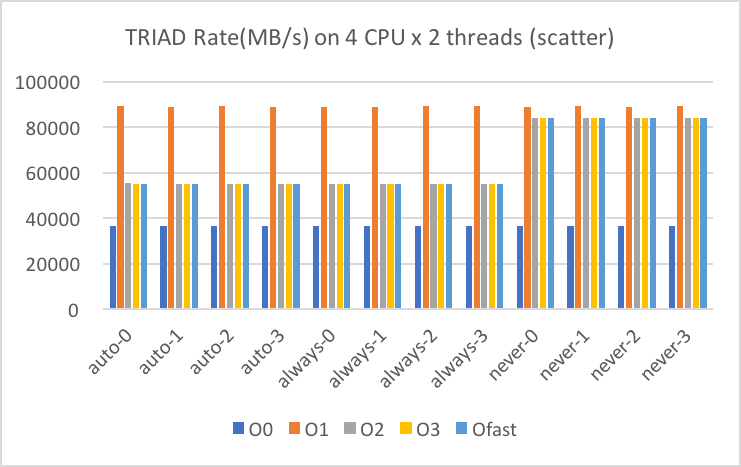
\includegraphics[width=0.45\textwidth]{figs/stream-ivy-scatter-4cpux2.pdf}
\caption{stream-ivy-scatter-4cpux2}
\label{fig:stream-ivy-scatter-4cpux2}
\end{figure}

図\ref{fig:stream-ivy-compact-1cpux8} と
図\ref{fig:stream-ivy-scatter-4cpux2} と
でPMlibが出力するHWPC Cache関係の数値を比較すると***
が読み取れる.



\section{Reminders}
Do not mix abbreviations of units: ``Wb/m\textsuperscript{2}'' or ``webers per square meter''.


Punctuate equations with commas or periods when they are part of a sentence, as in:
\begin{equation}
a+b=\gamma\label{eq}
\end{equation}

reference to the equation with numbers only \eqref{eq}.
you may use slash (~/~) in equation.
For figures, use the abbreviation ``fig.~\ref{fig}''.


\section*{Acknowledgment}

\section*{References}

citation first, followed by the original foreign-language citation \cite{b6}.

\bibliographystyle{jplain}
\bibliography{PMlib}
\end{document}




